\subsection{Package com.sirius.sequenziatore.server.service}
Questo \textit{package} conterrà tutti i \textit{service} necessari per le elaborazioni dei dati, ogni \textit{service} è associato con un rispettivo \textit{controller}.
\begin{figure}[H] \centering 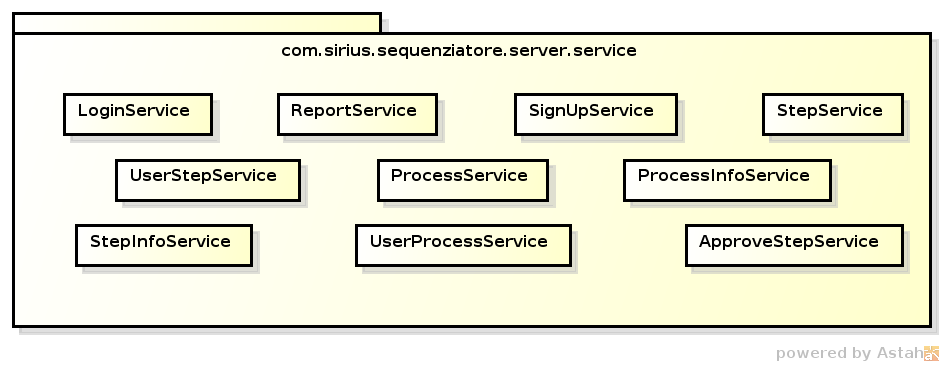
\includegraphics[width=%
\textwidth]
{./pack/serverService.png} \caption{Diagramma package service}
\end{figure}
\paragraph{LoginService}
	\begin{itemize}
		\item \textbf{Nome:} \texttt{LoginService};
		\item \textbf{Package:} \texttt{com.sirius.sequenziatore.server.service}
		\item \textbf{Descrizione:} Classe che permette la gestione della login di un utilizzatore del sistema, controllando che i dati inseriti riferiscano a un utente correttamente iscritto al sistema, ponendo attenzione se esso sia un \textit{process owner} o un utente normale;
		\item \textbf{Relazione con altre componenti:} la classe invoca i metodi delle classi:
		\begin{itemize}
			\item \texttt{com.sirius.sequenziatore.server.model.IDataAccessObject;}
			\item \texttt{com.sirius.sequenziatore.server.model.ITransferObject}
		\end{itemize}
	\end{itemize}
\paragraph{SignUpService}
	\begin{itemize}
		\item \textbf{Nome:} \texttt{SignUpService};
		\item \textbf{Package:}\texttt{ com.sirius.sequenziatore.server.service}
		\item \textbf{Descrizione:} Classe che permette la gestione della registrazione di un nuovo utente nel sistema, in quanto la correttezza dei dati inseriti viene controllata dalla parte client, dovrà inserire il nuovo utente e in caso di errore avvisare il controller;
		\item \textbf{Relazione con altre componenti:} la classe invoca i metodi delle classi:
		\begin{itemize}
			\item \texttt{com.sirius.sequenziatore.server.model.IDataAccessObject;}
			\item \texttt{com.sirius.sequenziatore.server.model.ITransferObject}
		\end{itemize}
	\end{itemize}
\paragraph{StepInfoService}
	\begin{itemize}
		\item \textbf{Nome:} \texttt{StepInfoService};
		\item \textbf{Package:}\texttt{ com.sirius.sequenziatore.server.service}
		\item \textbf{Descrizione:} Classe che fornisce lo scheletro di un passo, quindi andrà a fornire i dati da inserire per tale passo e altre informazioni;
		\item \textbf{Relazione con altre componenti:} la classe invoca i metodi delle classi:
		\begin{itemize}
			\item \texttt{ com.sirius.sequenziatore.server.model.IDataAccessObject;}
			\item \texttt{com.sirius.sequenziatore.server.model.ITransferObject}
		\end{itemize}
	\end{itemize}
\paragraph{ProcessInfoService}
	\begin{itemize}
		\item \textbf{Nome:} \texttt{ProcessInfoService};
		\item \textbf{Package:} \texttt{com.sirius.sequenziatore.server.service}
		\item \textbf{Descrizione:} Classe incaricata di recuperare lo scheletro di un processo, come ad esempio numero di passi o condizioni per il suo completamento;
		\item \textbf{Relazione con altre componenti:} la classe invoca i metodi delle classi:
		\begin{itemize}
			\item \texttt{com.sirius.sequenziatore.server.model.IDataAccessObject;}
			\item \texttt{ com.sirius.sequenziatore.server.model.ITransferObject}
		\end{itemize}
	\end{itemize}
\paragraph{ProcessService}
	\begin{itemize}
		\item \textbf{Nome:} \texttt{ProcessService};
		\item \textbf{Package:} \texttt{com.sirius.sequenziatore.server.service}
		\item \textbf{Descrizione:} Classe che gestisce i processi come ad esempio la creazione, la modifica e l' eliminazione degli stessi;
		\item \textbf{Relazione con altre componenti:} la classe invoca i metodi della classe:
		\begin{itemize}
			\item \texttt{com.sirius.sequenziatore.server.model.IDataAccessObject;}
		\end{itemize}
	\end{itemize}
\paragraph{StepService}
	\begin{itemize}
		\item \textbf{Nome:} \texttt{StepService};
		\item \textbf{Package:} \texttt{com.sirius.sequenziatore.server.service}
		\item \textbf{Descrizione:} Classe che permette di ottenere passi e dati a loro relativi;
		\item \textbf{Relazione con altre componenti:} la classe invoca i metodi della classe:
		\begin{itemize}
			\item \texttt{com.sirius.sequenziatore.server.model.IDataAccessObject;}
		\end{itemize}
	\end{itemize}
\paragraph{ApproveStepService}
	\begin{itemize}
		\item \textbf{Nome:} \texttt{ApproveStepService};
		\item \textbf{Package:} \texttt{com.sirius.sequenziatore.server.service}
		\item \textbf{Descrizione:} Classe che permette al process owner la gestione dei passi da approvare, quindi con questa classe si otterranno la lista di passi da approvare e si gestirà la approvazione o il rifiuto dei suddetti in base all' esito del process owner;
		\item \textbf{Relazione con altre componenti:} la classe invoca i metodi della classe:
		\begin{itemize}
			\item \texttt{com.sirius.sequenziatore.server.model.IDataAccessObject;}
		\end{itemize}
	\end{itemize}
\paragraph{UserProcessService}
	\begin{itemize}
		\item \textbf{Nome:} \texttt{UserProcessService};
		\item \textbf{Package:} \texttt{com.sirius.sequenziatore.server.service}
		\item \textbf{Descrizione:} classe che ottiene i dati di uno o più processi, ottiene lo stato di un utente per un processo ed inoltre gestisce la richiesta di un utente di iscrizione o disiscrizione a un processo;
		\item \textbf{Relazione con altre componenti:} la classe richiama i metodi della classe:
		\begin{itemize}
			\item \texttt{com.sirius.sequenziatore.server.model.IDataAccessObject;}
		\end{itemize}
	\end{itemize}
\paragraph{UserStepService}
	\begin{itemize}
		\item \textbf{Nome:} \texttt{UserStepService};
		\item \textbf{Package:} \texttt{com.sirius.sequenziatore.server.service}
		\item \textbf{Descrizione:} questa classe salva i dati inviati da un utente per un determinato passo nel database;
		\item \textbf{Relazione con altre componenti:} la classe richiama i metodi della classe:
		\begin{itemize}
			\item \texttt{ com.sirius.sequenziatore.server.model.IDataAccessObject;}
		\end{itemize}
	\end{itemize}
\paragraph{ReportService}
	\begin{itemize}
		\item \textbf{Nome:} \texttt{ReportService};
		\item \textbf{Package:} \texttt{com.sirius.sequenziatore.server.service}
		\item \textbf{Descrizione:} Classe che ottiene i dati per generare il report dell' utente riferito al processo richiesto;
		\item \textbf{Relazione con altre componenti:} la classe richiama i metodi della classe:
		\begin{itemize}
			\item \texttt{com.sirius.sequenziatore.server.model.IDataAccessObject;}
		\end{itemize}
	\end{itemize}

	